%!TEX root = thesis.tex
\chapter{Methodology}

	This chapter describes the methodology used to find the optimum configurations of the ASF. To study the electricity generation and building energy consumption, a 3D geometry of the room and solar facade is built using the Rhinoceros software \cite{Rhino}, and its parametric modelling plugin Grasshopper \cite{grasshopper}. The aquired data is then post-processed in Python \cite{python} to extract the configurations that minimise building energy consumption and maximise PV electricity production.

	\section{Thermal and Lighting Analysis}

		The building energy simulation is conducted using EnergyPlus \cite{energyplus} through the DIVA \cite{DIVA} interface. In EnergyPlus, the geometric solar facade is interpreted as an external shading system. Simulations are performed for a whole year at fixed angle positions, outputing hourly values of energy use for heating, cooling and lighting. Optimum positions can then be found by comparing the energy deman during every hour for all combinations. 

	\section{Radiation and PV Analysis}

		A solar radiance simulation is run in parallel using Ladybug \cite{roudsari2014ladybug},  which uses Radiance \cite{ward1994radiance} to determine the incident insolation on the solar facade. The approach enables to calculate solar irradiance on the modules with high spatial resolution including the effect of module mutual shading as seen in Figure \ref{fig:radiation}. The radiation is analysed for cumulative monthly hours for the whole year. The results are afterwards coupled to an electrical circuit simulation of thin-film PV modules with sub-cell level representation \cite{hofer2015PVSEC}. It is important to note that 

		\begin{figure}[H]
		\begin{center}
			\includegraphics[width=8cm, trim= 0cm 0cm 0cm 0cm,clip]{radiationanalysis.png}
			\caption{A simulation result showing module insolation from 11:00-12:00 on the 16 June for the used weather file and a specific module orientation.}
			\label{fig:radiation}
		\end{center}
		\end{figure}

	\section{Combined Evaluation}

	\section{Simulation Framework}
		A corresponding workflow can be seen in Figure \ref{fig:workflow}. 

		\begin{figure}[ht] %h can be omitted for better page layout
		\begin{center}
			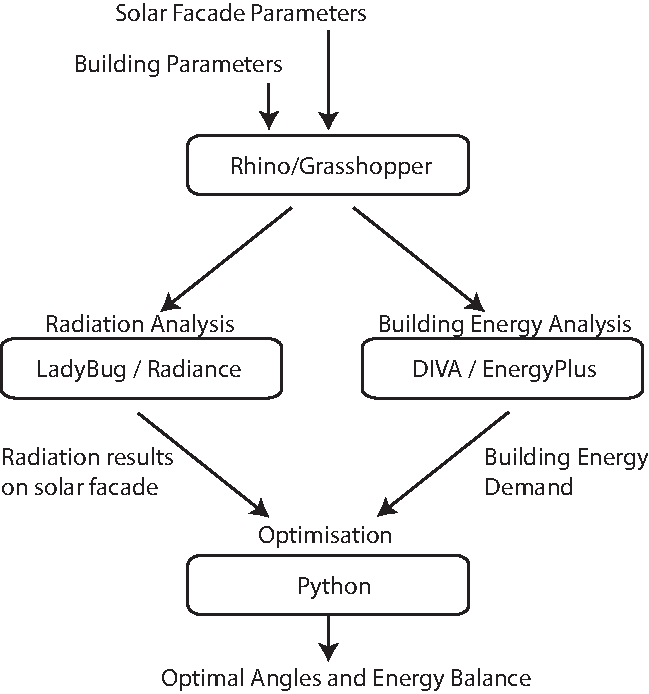
\includegraphics[width=0.75\textwidth, trim= 0cm 0cm 0cm 0cm,clip]{workflow_vertical}
			\caption{Work flow of the simulation framework}
			\label{fig:workflow}
		\end{center} 
		\end{figure}

	\section{Case Study}
		The solar facade consists of 400mm CIGS square panels that can rotate in two degrees of freedom. On the horizontal axis, the panels can move from 0$^{\circ}$ (closed) to 90$^{\circ}$ (open) position in steps of 22.5$^{\circ}$. In the vertical axis, it can move from 45$^{\circ}$ to -45$^{\circ}$ in 22.5$^{\circ}$ steps. Existing ASF systems \cite{nagy2015frontiers} have independently actuated panels and a continuous range of actuation, however for simplicity, we group all panels into one cluster that moves in unison. This leaves us with 25 possible dynamic configurations of the facade system. 

		The office environment is heated with a heatpump with an average COP of 5 and cooled with an average COP of 3. When required, the electric lighting consumption is 11.7 $W/m^2$. 

		A simulation of each possible dynamic configuration of the facade is run for each hourly timestep of the year using using a weather file for Kloten, Switzerland. %\cite{genevaweatherfile}. %The results are then post-processed in Python \cite{python} to extract the configurations that minimise building energy consumption and maximise PV electricity production.



